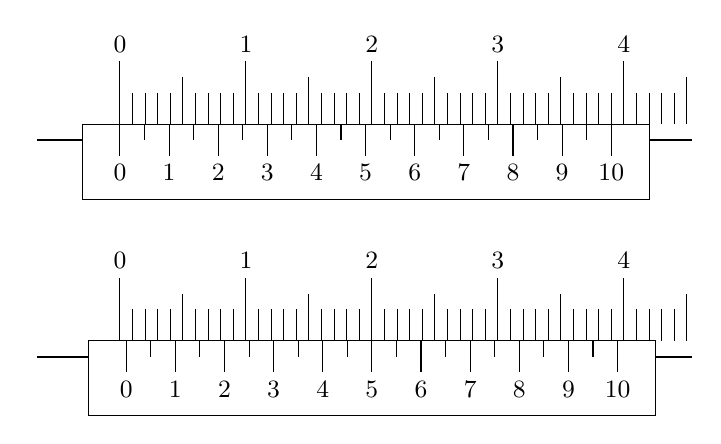
\begin{tikzpicture}%
  \node at (0, 0) {};
  \pgfmathsetmacro{\xscale}{0.16}
  \pgfmathsetmacro{\xstart}{30.}
  \pgfmathsetmacro{\y}{0.}
  
  {\small
  % Main scale.
  \draw[thick] (0,\y) -- (52*\xscale,\y);
  \foreach \x in {0,1,...,45}
  \draw[xshift=\xstart] (\x*\xscale,\y+0.2) -- (\x*\xscale,\y+0.6) {};
  \foreach \x in {0,5,...,45}
  \draw[xshift=\xstart] (\x*\xscale,\y+0.2) -- (\x*\xscale,\y+0.8) {};
  \foreach \x in {0,10,...,45}
  \draw[xshift=\xstart] (\x*\xscale,\y+0.2) -- (\x*\xscale,\y+1.0) node[anchor=south] {\pgfmathparse{0.1*\x}\pgfmathprintnumber{\pgfmathresult}};

  % Vernier scale
  \draw [fill=white,xshift=\xstart] (-3*\xscale,\y+0.2) rectangle (42*\xscale,\y-0.75);
  \foreach \x in {0,1,...,20}
  \draw[xshift=\xstart] (1.95*\x*\xscale,\y+0.2) -- (1.95*\x*\xscale,\y-0.) {};
  \foreach \x in {0,2,...,20}
  \draw[xshift=\xstart] (1.95*\x*\xscale,\y+0.2) -- (1.95*\x*\xscale,\y-0.2) node[anchor=north] {\pgfmathparse{0.5*\x}\pgfmathprintnumber{\pgfmathresult}};

  \pgfmathsetmacro{\y}{-2.75}

  % Main scale.
  \draw[thick] (0,\y) -- (52*\xscale,\y);
  \foreach \x in {0,1,...,45}
  \draw[xshift=\xstart] (\x*\xscale,\y+0.2) -- (\x*\xscale,\y+0.6) {};
  \foreach \x in {0,5,...,45}
  \draw[xshift=\xstart] (\x*\xscale,\y+0.2) -- (\x*\xscale,\y+0.8) {};
  \foreach \x in {0,10,...,45}
  \draw[xshift=\xstart] (\x*\xscale,\y+0.2) -- (\x*\xscale,\y+1.0) node[anchor=south] {\pgfmathparse{0.1*\x}\pgfmathprintnumber{\pgfmathresult}};

  % Vernier scale
  \draw [fill=white,xshift=\xstart] (-3*\xscale+0.5*\xscale,\y+0.2) rectangle (42*\xscale+0.5*\xscale,\y-0.75);
  \foreach \x in {0,1,...,20}
  \draw[xshift=\xstart] (1.95*\x*\xscale+0.5*\xscale,\y+0.2) -- (1.95*\x*\xscale+0.5*\xscale,\y-0.) {};
  \foreach \x in {0,2,...,20}
  \draw[xshift=\xstart] (1.95*\x*\xscale+0.5*\xscale,\y+0.2) -- (1.95*\x*\xscale+0.5*\xscale,\y-0.2) node[anchor=north] {\pgfmathparse{0.5*\x}\pgfmathprintnumber{\pgfmathresult}};
  }
\end{tikzpicture}
